\documentclass{chi2009}
\usepackage{times}
\usepackage{url}
\usepackage{graphics}
\usepackage{color}
\usepackage[pdftex]{hyperref}
\usepackage[T1]{fontenc}

\hypersetup{%
pdftitle={Deep Q Learning with Flappy Bird},
pdfauthor={Ryan Drapeau, Sonja Khan, Aaron Nech},
pdfkeywords={reinforcement learning, neural networks, DQN, flappy bird},
bookmarksnumbered,
pdfstartview={FitH},
colorlinks,
citecolor=black,
filecolor=black,
linkcolor=black,
urlcolor=black,
breaklinks=true,
}
\newcommand{\comment}[1]{}
\definecolor{Orange}{rgb}{1,0.5,0}
\newcommand{\todo}[1]{\textsf{\textbf{\textcolor{Orange}{[[#1]]}}}}

\pagenumbering{arabic}  % Arabic page numbers for submission.  Remove this line to eliminate page numbers for the camera ready copy

\begin{document}
% to make various LaTeX processors do the right thing with page size
\special{papersize=8.5in,11in}
\setlength{\paperheight}{11in}
\setlength{\paperwidth}{8.5in}
\setlength{\pdfpageheight}{\paperheight}
\setlength{\pdfpagewidth}{\paperwidth}

% use this command to override the default ACM copyright statement
% (e.g. for preprints). Remove for camera ready copy.
\toappear{Submitted to CSE 571 (Fall '15) as the final paper.}

\title{Deep Q Learning with Flappy Bird}
\numberofauthors{3}
\author{
  \alignauthor Ryan Drapeau\\
    \affaddr{University of Washington}\\
    \email{drapeau@\footnotemark[1]}
  \alignauthor Sonja Khan\\
    \affaddr{University of Washington}\\
    \email{sonjak3@\footnotemark[1]}
  \alignauthor Aaron Nech\\
    \affaddr{University of Washington}\\
    \email{necha@\thanks{@cs.washington.edu}}
}

\maketitle

\begin{abstract}
Deep neural networks have recently been used to successfully learn policies for popular video games. We applied similar methods to a popular mobile game: Flappy Bird by implementing a novel reinforcement learning algorithm. We first started with a simplified model of the game consisting of only two features, and then we increased the complexity by generalizing the input to the pixels on the screen. We present our methods and results for training a Flappy Bird agent to maximize game score.
\end{abstract}

\keywords{reinforcement learning, neural networks, DQN, flappy bird}

\section{Introduction}

One of the main goals of reinforcement learning is having an agent learn from experience in a specific environment. In this paper we will explore the direct application of deep reinforcement learning to popular games and analyze the challenges with the Deep Q Learning algorithm in this setting.

\section{Background}

We settled on the popular game of Flappy Bird. Flappy Bird is a mobile game developed by Nguy$\hat{\text{\~e}}$n H\`a \DH\^ong in 2013 and quickly rose to be one of the most successful mobile games of all time \cite{nguyen2013flappy}. The game has a simple side-scrolling environment where the goal is to navigate the bird through a never-ending series of pipes. The player is reset back to the beginning if he or she collides with the ground or with the side of a pipe. This game was chosen because of its simplicity in its action and state spaces. The action space consists of 2 actions: \{jump, do nothing\} as there is an external factor of gravity that pulls the user down towards the ground. The state space is also simple because there are only two actors on the screen, the bird and a pipe.

Further work has explored the domain of Super Mario Bros. and many other related games using deep neural networks \cite{murphy2013first}. This work ignored the current ``score'' of the game and instead rewarded the network based on the RAM state of the emulator. The idea behind this is that in general, increasing numbers in memory are a good indicator of success in simple games like Mario, i.e., score, position, time alive, etc.

\section{Related Work}

Much work has been done in the field of reinforcement learning, one notable example is TD-gammon, which was a program that learned to play backgammon through temporal difference learning \cite{tesauro1995temporal}. Temporal difference learning was successful in this application and was able to produce a network that achieves master level play of the game. There has also been recent work by Google's Deepmind with Deep Q Learning being used to obtain expert level play in several ATARI games \cite{mnih2013playing}. Google was able to utilize the same network structure across 7 different games, including Beam Rider, Breakout, Pong, etc. The input to their network was the state of the screen (> 28,000 features), which was then passed through many convolutional and pooling layers before reaching the output layer. While their work was highly successful, they trained their network on a cluster of GPUs for multiple weeks, which is out of the scope for this project. Many related works followed from Deepmind's paper on the ATARI domain of games. We chose not to explore this domain because of the vast complexity of the games, which may have introduced additional complexity into our 6-week project.

\section{Methods}

We chose JavaScript as it would allow us rapid development with the ability to quickly iterate based on visuals produced in the browser. Since the environment was easy to set up and reproduce across a wide variety of machines, we found that a combination of browser technologies and NodeJS were excellent for our requirements. The wide availability of libraries for neural network and Deep-Q Learning also steered our choice towards JavaScript.

\subsection{Existing Flappy Bird Implementations}

As a first priority, we needed to be able to simulate the game of Flappy Bird such that we could produce state vectors to feed our Neural Network implementation to train within the DQN framework. We wished to do this quickly -- faster than playing at real time -- such that our bottleneck in training was solely the neural network training and not the game itself. To accomplish this we first looked toward scavenging existing Flappy Bird implementations written in JavaScript. The results were very poor. Many implementations strongly coupled rendering to game logic. For example many implementations coupled collision to the browser Document Object Model (DOM), by utilizing intrinsic bounding box collision approximations provided by representation of game actors as DOM nodes \cite{floppybird}. Other implementations utilized Cascading Style Sheet (CSS) transitions to linearly interpolate movement of actors \cite{clumsybird}. This made it exceedingly difficult to separate logic from rendering such that we could run the simulation quickly.

\begin{figure}[t]
\begin{center}

\includegraphics[width=0.8\columnwidth]{figs/conv.jpg}
\vspace*{-0.05in}
\caption{Semantic pixel map input to the network.}
\label{fig:flappy_game}
\end{center}
\end{figure}

\subsection{Flappy Bird Simulator}

Ultimately, we opted for creating our own Flappy Bird implementation which prioritized complete separation of state and logic from rendering. The simulation was designed such that it has three main operations:

\begin{description}
    \item[tick()] - Moves the simulation forward by one frame. This advances the simulation and recalculates the simulation state.
    \item[getState()] -  Obtains the current state of the simulation. Such as bird actor position, pipe position, and down sampled semantic pixel maps.
    \item[reset()] - Resets the simulation to the initial state. Ticking the simulation has a chance of doing this as well. For example, if the bird hits a pipe or the ground, the simulation resets.
\end{description}

\subsection{Semantic Pixel Maps}

Our simulation provides the ability to quickly sample Semantic Pixel Maps where a pixel is given a value to indicate if it belongs to a Pipe or Bird, see Figure \ref{fig:flappy_game}. These proto-rendered screens are quick to sample and provide more meaningful representations for learning. Initial DQN testing involved feeding more meaningful states to the DQN framework. For example, a successful training session was obtained by feeding the two dimensional distance vector between the bird and the next pipe as input state to the DQN. As we progressed in development, our goal was to give more and more vague features to the DQN. In this way we trade off training time (on the order of days for simple features such as the distance vector, and on the order of weeks for semantic pixels), for more generality in learning (can the agent learn with fewer exact features, more as humans do).

\subsection{ConvNetJS and DQN Framework}

We chose to use and extend an existing JavaScript implementation of Neural Networks written by Karpathy, ConvNetJS \cite{karpathygoogle}. This allows us to focus on the learning implementation, rather than debug Neural Network implementations. On top of this we found a well written base for Deep Q Learning that was written on top of ConvNetJS. This implementation lacked the ability for us to input pixel maps and connect Convolutional Neural Network layers, but we were able to implement these additions. The DQN Framework provided a simple interface for specifying neural network parameters and structure, and feeding input for forward and backward propagation. We easily connected this framework to our later developed Parameter File system for describing the totality of DQN parameters on a higher level of abstraction (reward function, input function, training constraints, and neural network structure). These extensions allow us to more easily connect the DQN framework to our Flappy Bird architecture. See Figure \ref{fig:architecture} for a deeper look into the interactions between the different modules.

\begin{figure}[t]
\begin{center}
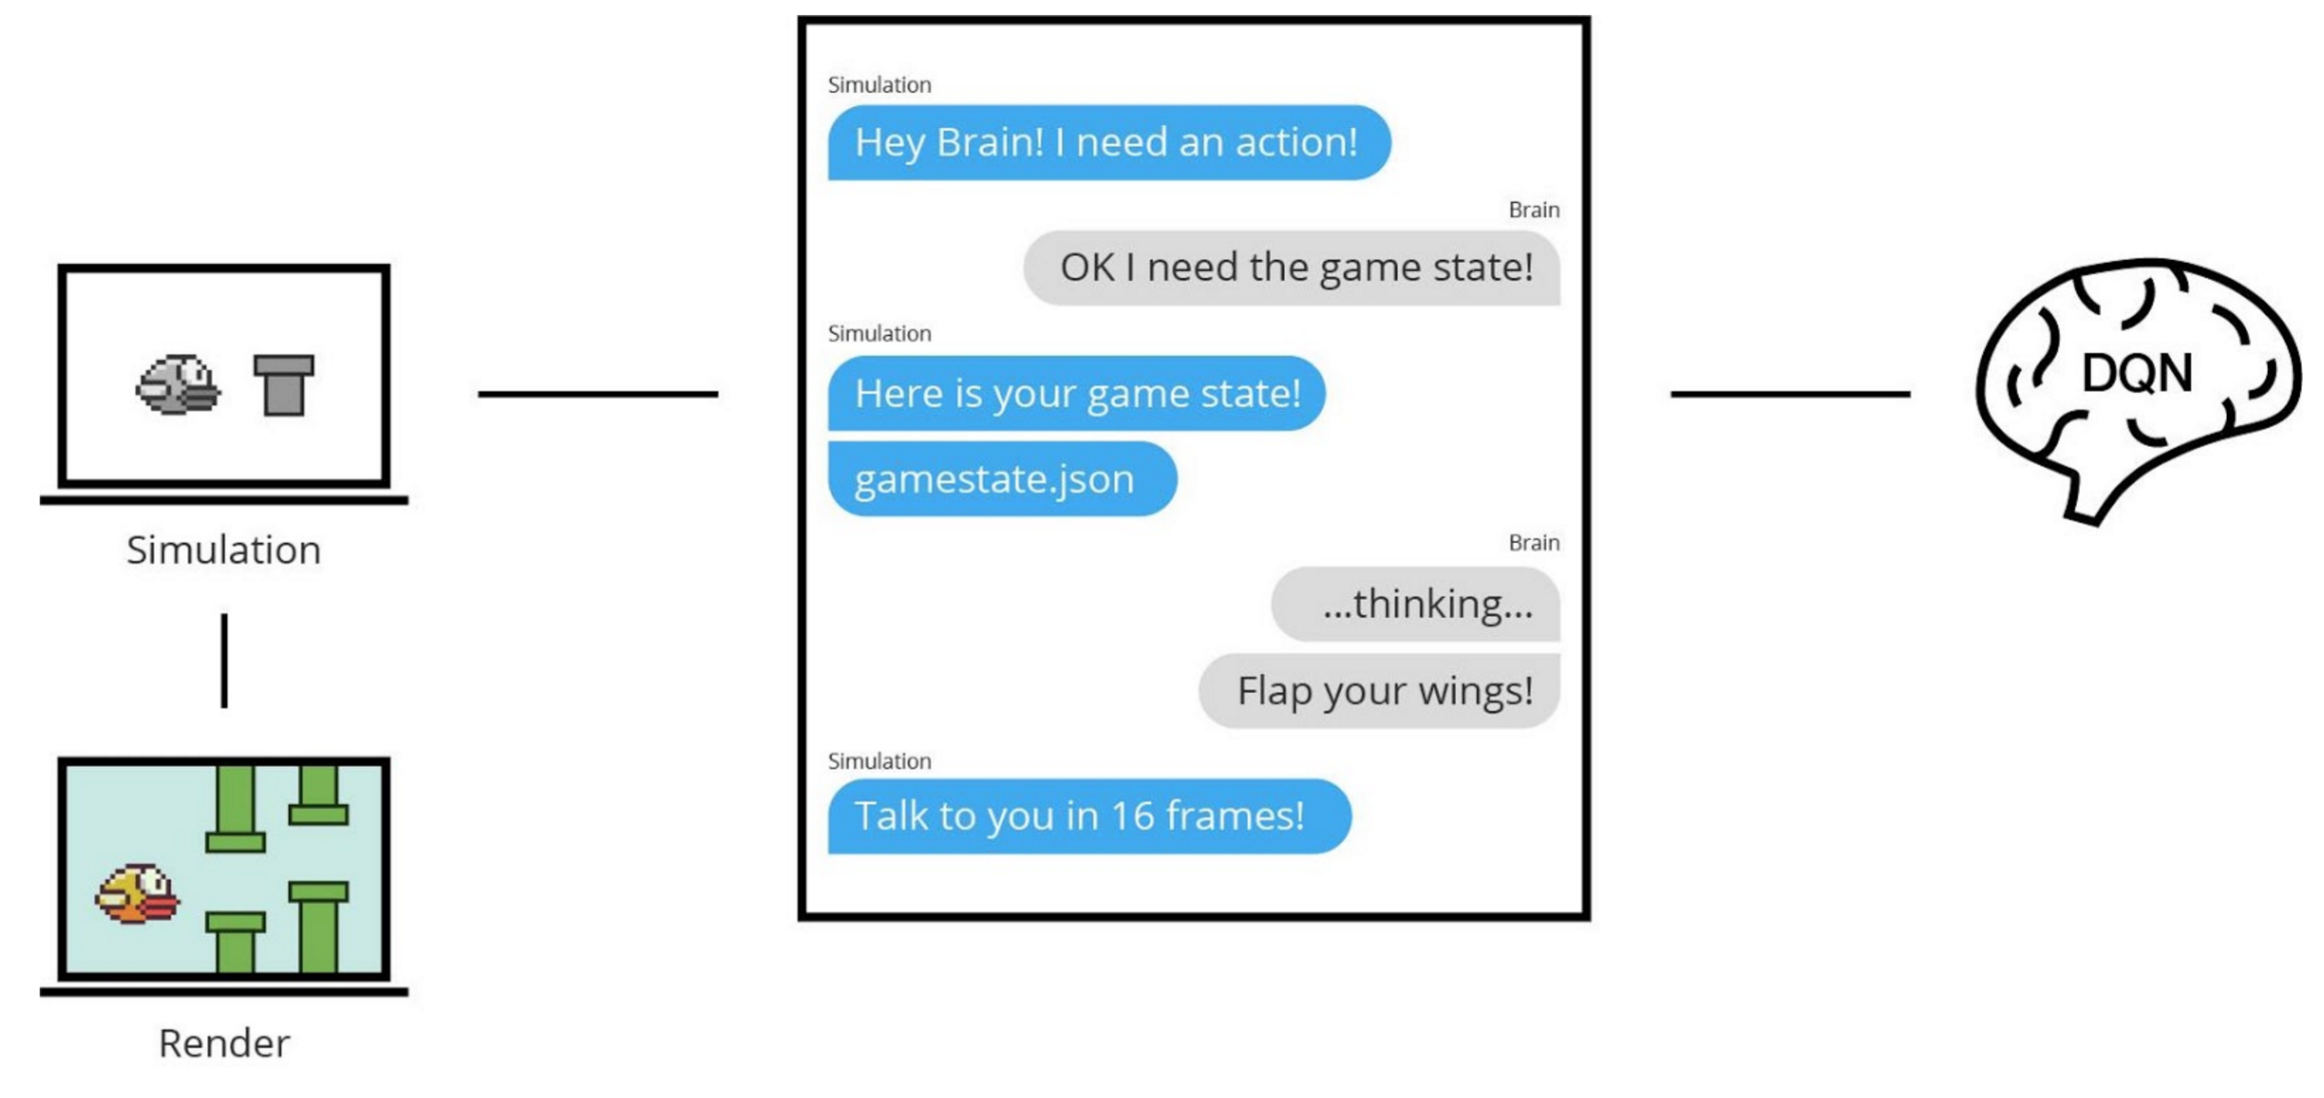
\includegraphics[width=\columnwidth]{figs/architecture.png}
\vspace*{-0.25in}
\caption{Basic architecture of the simulation and network.}
\label{fig:architecture}
\end{center}
\end{figure}

\subsection{Simulation-DQN Adapter}

Once we set up the simulation and DQN framework, we needed to connect the two in a modular way. We created a simple adapter which allows us to provide the functionality the DQN framework expects given the simulation the adapter has access to. We then pass the adapter to the DQN training framework, and the DQN framework accesses the resources it requires from the adapter. The adapter later becomes a wrapper over our Parameter File system so we can specify reproducible training sessions in single files.

\subsection{Simulation Timer}

Finally, a timer class is required to hook all these pieces together in a synchronized way. The timer class runs the DQN code at a specified interval that is disjoint from the simulation interval. It also ticks the simulation at a specific interval. For example, the timer allows us to tick forward the DQN Neural Network every Nth frame of the simulation, where $N$ does not always equal $1$. This gives us the freedom to parameterize how often the DQN can provide an action to the simulation.

\subsection{Parameter Files}

Parameter files allow us to specify the entirety of parameters needed to reproduce a specific training session. For this project we created over $50$ parameter files testing different reward functions, input state (e.g. Semantic Pixels vs. Pipe location), and network parameters (e.g. learning rate, random action time-frame). The Adapter described above produces much of it's input to the DQN framework through these parameter files. For example when the DQN framework requests network parameters from the adapter, the adapter simply looks them up in the current parameter file.

\subsection{Trainer}

As an optimization, we wrote a trainer that can be run in NodeJS (a fast JIT-compiled JavaScript interpreter), such that we can run simulations over long periods of times without keeping a browser open. NodeJS also performs better than the browser counterpart in our tests. The training program takes as input a parameter file, and outputs trained network weights.

\begin{figure}[t]
\begin{center}
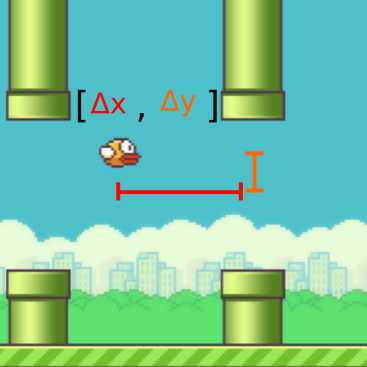
\includegraphics[width=0.8\columnwidth]{figs/state.png}
\vspace*{-0.05in}
\caption{Input state to the network was simply $\left[\Delta X, \Delta Y \right]$. Other networks tried to incorporate $dx$ and $dy$ unsuccessfully.}
\label{fig:state}
\end{center}
\end{figure}

\subsection{Browser Display and Debugger}

We created a browser based system which can train and test specific parameter files. Since the browser implementation is slower, we ultimately use it as a way to test our the results of the NodeJS training program. The browser system allows uploading of trained weight files for specific parameter sets to visually inspect the actions of the trained DQN agent.

\subsection{Rendering}

ReactJS, a UI library created by Facebook, was utilized to create our Flappy Bird browser system. React allowed us to specify various parts of the system as React Components which are decomposable to create the full system. We created a Flappy Bird renderer, which takes as input the Flappy Bird simulator described above, and outputs a canvas display of the game state which strongly mimics the original game. This allows us to visually inspect trained agents, and create demonstrations of our work.

\begin{figure}[t]
\begin{center}

\includegraphics[width=0.8\columnwidth]{figs/close.png}
\vspace*{-0.09in}
\caption{The network would play ``pixel-perfectly'', which would sometime perform moves a human would never attempt.}
\label{fig:close}
\end{center}
\end{figure}

\section{Results}

We now present the results of our experiments. Our first approach was feeding the neural network hand-engineered features as input (see Figure \ref{fig:state}), experimenting with several reward functions. Punishing heavily for death or rewarding positively for staying alive yielded poor results. In these cases, the bird learned that flapping was the optimal action and flew to the top. Giving a high reward for scoring (making it through a pipe) resulted in the bird successfully learning to clear pipes. See Figure \ref{fig:plot} for a plot of the reward function over time for a brain with 2 fully connected layers running for 2 million iterations.

In order to capitalize on the power of deep q learning, we generalized the input state given to the brain. We now describe our most successful attempt. Our new input to the neural network was a down-sampled semantic pixel map with dimensions 40 x 46 x 1. The first hidden layer convolves 2 5 x 5 filters with stride 1, followed by a 4 x 4 pooling layer with stride 4. The next layer convolves 4 5 x 5 filters with stride 1, again followed by a 4 x 4 pooling layer with stride 4. The final hidden layer is fully connected. After 600k training iterations, the smooth-ish reward was approximately 1.9. Testing with this brain showed the bird attempting to fly towards the pipe opening, but failing to pass through without dying.

\begin{figure}[t]
\begin{center}
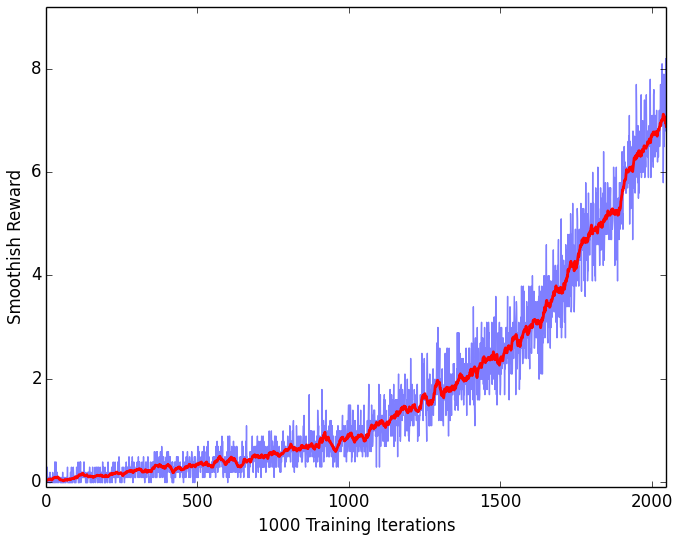
\includegraphics[width=\columnwidth]{figs/smooth_reward.png}
\vspace*{-0.09in}
\caption{The networks performance as it was trained over 2 million iterations (a few hours for this network structure).}
\label{fig:plot}
\end{center}
\end{figure}

\section{Discussion}

Our ultimate goal was to train Flappy Bird by just passing in the game pixels as input. We approached this by gradually increasing the complexity of our input state. There was a lot of parameter tweaking during the first step of training to get a working agent. We were initially using the Euclidean pixel distance between the bird and nearest pipe as our state input. These were large values in the range [0, 320] for x and [-184, 184] for y, and because our network has a positive feedback loop, the values increased exponentially and overflowed. We solved this issue by dividing the x and y distance by the width and height of the game respectively.

After this fix, the bird was able to learn, but we now faced the problem that it always learned to fly to the top. We tried increasing the training time from 200k to 600k with no change in results. We deduced that the bird was not able to fly through the first pipe often enough, or that the reward for making it through the pipe was not high enough to shift the weights of our network encourage this behavior in future. We increased our threshold to start learning so the network would have a larger sample of states before starting to apply policy actions, and increased the reward for scoring to 100.0 from 5.0. Our agent was able to learn to beat the game reasonably well with 600k iterations.

Generalizing our input state proved to be a challenge. Our input state was now 1840 features, which resulted in a significant time increase for the computation of each iteration. We used convolution layers in our network to take advantage of shared weights, and added pooling layers to further down-sample the input. Training for 600k iterations took 2 days, compared to 1 hr for the hand-engineered input approach. At the end of this training, the bird had learned to flap in the general direction of the pipe opening, but did not learn to score. We trained multiple agents, modifying parameters such as the reward function, down-sampling ratio, training iterations, experience replay, and network layers, but none were able to clear the first pipe. We found that down-sampling the image too much yielded extremely poor results, and that including a large number of convolution filters slowed down the computation by an order of magnitude. We believe that our networks needed many more training iterations. Similar previous work on this topic has demonstrated results after training for weeks on a cluster of GPUs.

\section{Future Work}

We have left many directions for future work. Successfully training a network that only takes as input the state of the screen (with pipes and bird differentiated) would be a great direction after this paper. Following that, the next step would be to simply pass the raw pixels as input to the network instead of supplying information for the difference between a bird and a pipe. Unfortunately, both of these directions would require substantial training on a GPU or significantly longer time using our setup described in this paper. For reference, Deepmind trained their networks for 2 weeks on a GPU in order to reach ``super-human'' levels of performance \cite{mnih2013playing}.

\section{Conclusion}

In this paper we have shown our implementation of a reinforcement learning framework in the specific domain of Flappy Bird. We looked at related work in the domain of ATARI games, presented our efficient implementation to Flappy Bird, and walked through some of the training efforts that we took to attain great performance in the game.

\section{Acknowledgments}

We would like to thank Dieter Fox and Arunkumar Byravan for helping us throughout the project with guidance and feedback.

\bibliographystyle{abbrv}
\bibliography{references}

\end{document}
